\documentclass{article} 
\usepackage{pgfplots} 
\begin{document} 

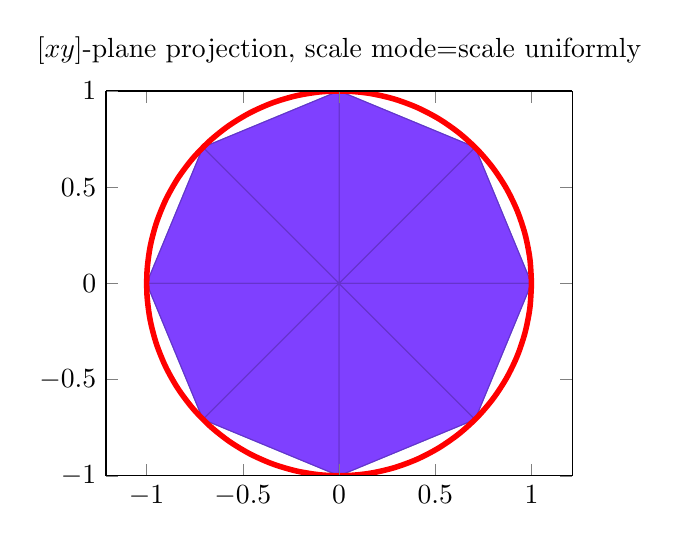
\begin{tikzpicture}
\begin{axis} [width=7.5cm, scale mode=scale uniformly, view={0}{90}, title={$[xy]$-plane projection, scale mode=scale uniformly}]
\addplot3 [surf, z buffer=sort, samples=5, variable=\u, variable y=\v, domain=0:180, y domain=0:360,
           colormap/cool] ({cos(u)*sin(v)}, {sin(u)*sin(v)}, {cos(v)});
\addplot3 [domain=0:360, samples=50, smooth, variable=\t, samples y=0,line width=2pt, red] ({cos(t)}, {sin(t)}, {2});
\end{axis}
\end{tikzpicture}

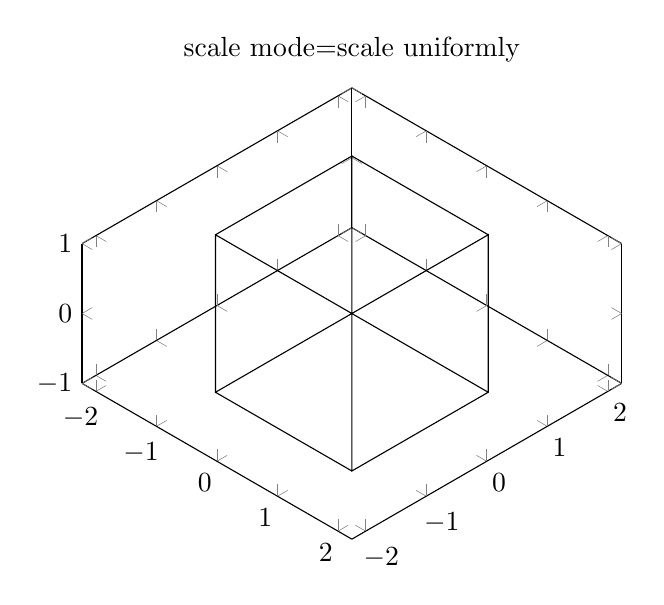
\begin{tikzpicture}
\begin{axis}[scale mode=scale uniformly, title={scale mode=scale uniformly},view={45}{35.26}]
\addplot3 [mark=cube, mark size=2cm] coordinates {(0,0,0)};
\end{axis}
\end{tikzpicture}
\end{document} 
